\documentclass{./llncs2e/llncs}
% \usepackage[printonlyused]{acronym} 
\usepackage{graphicx}
\usepackage{fixltx2e}
\usepackage[nolist,nohyperlinks]{acronym}

% 
% Title 
% 

\begin{document}
\title{Human's Cloud}
\titlerunning{Human's Cloud}
\toctitle{Human's Cloud}

\subtitle{A federated community cloud served by a P2P overlay network on top of the web platform}
\author{David Dias, david.dias@computer.org}
\authorrunning{David Dias}
\tocauthor{David Dias}
\institute{Lisbon Tech, University of Lisbon}

\maketitle


% ^^^^^^^^^^^^^^^^^^^^^^^^^^^^^^^^^^^^^^^^^^^^^^^^^^^^^^^^^^^^^^
% ~~~~~~~~~~~~~~~~~~~~~~~~~~~~~~~~~~~~~~~~~~~~~~~~~~~~~~~~~~~~~~
% ______________________________________________________________

% 
% Abstract 
% 

\begin{abstract}
Grid computing has been around since the 90's, its fundamental basis is to use idle resources in geographically distributed systems in order to maximize its efficiency, giving researchers access to computational resources to perform their jobs(e.g. studies, simulations, rendering, data processing, etc). This approach quickly grew into non grid environments, causing the appearance of projects such as SETI@Home or Folding@Home, that use volunteered shared resources and not only institution-wide data centers as before, creating the concept of Public Computing. Today, after having volunteering computing as a proven concept, we face the challenge of how to create a simple, effective, way for people to participate in this community efforts and even more importantly, how to reduce the friction of adoption by the developers and researchers to use this resources for their applications. This work explores current ways of making an interopable way of end user machines to communicate, using new Web technologies, creating a simple API that's familiar to those used to develop applications for the Cloud, but with resources provided by a community and not by a company or institution.

\end{abstract}



% ^^^^^^^^^^^^^^^^^^^^^^^^^^^^^^^^^^^^^^^^^^^^^^^^^^^^^^^^^^^^^^
% ~~~~~~~~~~~~~~~~~~~~~~~~~~~~~~~~~~~~~~~~~~~~~~~~~~~~~~~~~~~~~~
% ______________________________________________________________

% 
% Keywords 
% 

\begin{keywords}
Cloud Computing, Peer-to-peer, Voluntary Computing, Cycle Sharing, Decentralized Distributed Systems, Web Platform, Javascript, Fault Tolerance, Reputation Mechanism, 
\end{keywords}



% ^^^^^^^^^^^^^^^^^^^^^^^^^^^^^^^^^^^^^^^^^^^^^^^^^^^^^^^^^^^^^^
% ~~~~~~~~~~~~~~~~~~~~~~~~~~~~~~~~~~~~~~~~~~~~~~~~~~~~~~~~~~~~~~
% ______________________________________________________________

% 
% Introduction
% 

\section{Introduction}

%TODO Describe how problems are in interpreted and solved with algorithms based in the laws of nature (evolutionary computing and so on)

% \subsection{Cloud Computing}

% \subsection{Peer-to-Peer}


  ``An application is peer-to-peer if it aggregates resources at the network’s edge, and those resources can be anything. It can be content, it can be cycles, it can be storage space, it can be human presence.'', C.Shirky \cite{Shirky.}


% \subsection{Web platform}







% ^^^^^^^^^^^^^^^^^^^^^^^^^^^^^^^^^^^^^^^^^^^^^^^^^^^^^^^^^^^^^^
% ~~~~~~~~~~~~~~~~~~~~~~~~~~~~~~~~~~~~~~~~~~~~~~~~~~~~~~~~~~~~~~
% ______________________________________________________________

% 
% Objectives
% 

\section{Objectives}





% ^^^^^^^^^^^^^^^^^^^^^^^^^^^^^^^^^^^^^^^^^^^^^^^^^^^^^^^^^^^^^^
% ~~~~~~~~~~~~~~~~~~~~~~~~~~~~~~~~~~~~~~~~~~~~~~~~~~~~~~~~~~~~~~
% ______________________________________________________________

% 
% Related work
% 

\section{Related Work}
The purpose of this section is to show the state of the art of the research topics, more relevant to our proposed work, namely: Volunteer Computing, Cloud Computing, P2P Networks and the Web Platform
%%TODO: Describe what's coming stating section numbers

% 
%---------{Cloud computing and Open Source Cloud Platforms}-------
% 
\subsection{Cloud computing and Open Source Cloud Platforms}
%TODO More traditional known clouds EC2, AZURE, App Engine, ETC
%TODO openstack http://www.openstack.org/
% Ref links 
% http://www.openstack.org/summit/openstack-summit-hong-kong-2013/session-videos/presentation/ibm-keynote-managing-the-next-era-of-computing-with-an-open-cloud-architecture
% http://www.openstack.org/summit/openstack-summit-hong-kong-2013/session-videos/presentation/getting-started-with-openstack
%  
%TODO opencloud














% 
%---------{Volunteered resource sharing}--------------------------
% 
\subsection{Volunteered resource sharing}
%TODO 


% Acronymns        
% Application-level networks (ALN) 

% This is perfect to define the problem
% 
% Distributed evolutionary computing system based on web browsers with JavaScript
% Jerzy Duda and Wojciech Dłubacz
% Algorithms based on laws of nature:
% Evolutionary Algorithm - EA
% Simulated annealing - SA
% Colony optimization - ACO
% Particle swarmn optimization - PSO
% Artificial Bee Colonies - ABC
        
% You can divide the algoritms into two sets:
% Single Solution in each iteration
% Set of solutions, often refered as population

% You can decrease the computation time with metaheuristics
                  
% Models for distributed computation:
% Global parallelization model - One population sharded in small sets computed by several slaves
% Island Model - The population is divided in subpopulation that can run in heterogeneous machines (this is the most common in distributed computing)
% Master-Salve Model - One central pop that communicates and collects data from others              




\subsubsection{3.2.1 Hybrid and Community Clouds}
%TODO  * Computational Grids - TeraGrid, ChinaGrid and APACGrid
%TODO  * Data Grids - LHCGrid GriPhyN
%TODO  * Interaction Grids (focus on collaborative visualization) - AccessGrid
%TODO  * Knowledge Grids (knowledge acquisition)
%TODO  * Utility Grids (provide all grids services)


% User Centric Community Clouds 
% João Paulo Barraca · Alfredo Matos · Rui L. Aguiar

% Bla bla bla cloud is cheap, lack of control of data bla bla bla
% "User Centric Clouds" term appears in chapter 5  
% "A cloud system that uses user-centric technology can put the user back in the driver seatof his data,"
% It focus on users giving to the community the same services as the cloud providers do in a "common API"
% This is not a pure P2P thing



\subsubsection{3.2.2 Cycle and Storage Sharing, using Volunteer Computing Systems}
%TODO Here is more about projects, not about algorithms (SETI, freenet, etc) %TODO  Kazaa, napster, Seti, foldings, afins




\subsubsection{3.2.3 Peer-to-Peer Networks and Architectures -}  
Efficient resource discovery mechanisms are fundamental for a distributed system success, such as grid computing, cycle sharing or web application infrastructures\cite{Ranjan2006}, although in the centralized model, by keeping data bounded inside a data center, we have a stable and scalable way for resource discovery, this does not happen in a P2P network, where peers churn rate can vary greatly, there is no way to start new machines on demand for high periods of activity, the machines present are heterogeneous and so is their Internet connectivity, creating an unstable and unreliable environment. To overcome this challenges, several researches have been made in order to optimize how data is organized across all the nodes, improving the performance, stability and the availability of resources. The following paragraphs will describe the current state of the art P2P organizations, typically categorized in P2P literature as Unstructured or Structured\cite{Milojicic2003}, illustrated in Figure ~\ref{fig:Different types of P2P Overlay networks organizations}.

\begin{figure}[bh!]
  \begin{center}
    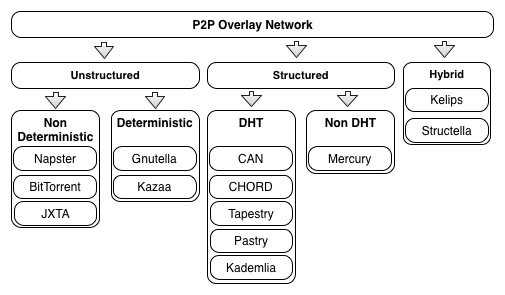
\includegraphics[width=\textwidth]{./img/p2porganizations.jpg}
  \end{center}
  \caption{Different types of P2P Overlay networks organizations}
  \label{fig:Different types of P2P Overlay networks organizations}
\end{figure}


\paragraph{\textbf{Unstructured -}} % (fold)
\label{par:Unstructured}

We call `Unstructured' to a P2P system that doesn't require or define any constraint for the placement of data, these include Napster, Kazaa and Gnutella, famous for it's file sharing capabilities, where nodes can share their local files directly, without storing the file in any specific Node. There is however a `caveat' in the Unstructured networks, by not having an inherent way of indexing the data present in the network, performing a lookup results of the cost of asking several nodes the whereabouts of a specific file or chunk of the file, creating a huge performance impact with an increasing number of nodes. In order to overcome this, Unstructured P2P networks offer several degrees of decentralization, one example is the evolution from Gnutella 0.4\cite{Definition2003} to Gnutella 0.6 \cite{T.Klingberg2002}\cite{Ripeanu2002a}, which added the concept of super nodes, entities responsible for storing the lookup tables for the files in parts of the network they are responsible for, increasing the performance, but adding centralized, single points of failure. 
\cite{Ranjan2006} classifies Unstructured networks into two types: deterministic and non-deterministic, defining that in a deterministic system, we can calculate before hand the number of hops needed to perform a lookup, knowing the predefined bounds, this includes systems such as Napster and BitTorrent\cite{Cohen2009}, in which the file transfers are decentralized, the object lookup remains centralized, keeping the data for the lookup tables stored in one place, which can be gathered by one of two ways : (i) peers inform directly the index server the files they have; or (ii) the index server performs a crawling in the network, just like a common web search engine, this gives this network a complexity of O(1) to perform a search, however systems like Gnutella 0.6, which added the super node concept, remain non deterministic because it's required to execute a query flood across all the super nodes to perform the search.

% paragraph Unstructured and Non-Deterministic (end)

\paragraph{\textbf{Structured with Distributed Hash Tables -}} % (fold)
\label{par:Structured with Distributed Hash Tables}

Structured P2P networks have an implicit way of allocating nodes for files and replicas storage, without the need of having any specie of centralized system for indexing, this is done by taking the properties of a cryptographic hash function \cite{Bakhtiari}\cite{Kargerl}\cite{Preneel1999}, such as SHA-1\cite{D.Eastlake3rdMotorola;P.JonesSystems2001}, which applies a transformation to any set of data with a uniform distribution of possibilities, creating an index with O(log(n)) peers, where the hash of the file represents the key and gives a reference to the position of the file in the network.
DHT's such as Chord\cite{Stoica2001}, Pastry\cite{Rowstron2001} and Tapestry\cite{Zhao2001}, use a similar strategy, mapping the nodes present in the network inside an hash ring, where each node becomes responsible for a segment of the hash ring, leveraging the responsibility to forward messages across the ring to his `fingers'(nodes that it knows the whereabouts). Kademlia\cite{Maymounkov} organizes it's nodes in a balanced binary tree, using XOR as a metric to perform the searches, while CAN\cite{Handley} introduced and a several dimension indexing system, in which a new node joining the network, will split the space with another node that has the most to leverage.
Evaluating the DHT Structured P2P networks raises identifiable issues/challenges, that result as the trade-off of not having an centralized infrastructure, responsible for railing new nodes or storing the meta-data, these are: (i) generation of unique node-ids is not easy achievable, we need always to verify that the node-id generated doesn't exist, in order to avoid collisions; (ii) the routing table is partitioned across the nodes, increasing the lookup time as it scales.
Table \ref{table:Complexity of structured P2P systems using a DHT}, showcases a comparison of the studied DHT algorithms.

\begin{table}
  \begin{tabular}{| p{1.3cm} | p{1.6cm} | p{1.9cm} | p{1.8cm} | p{1.6cm} | p{1.8cm} | p{1.8cm} |}
    \hline                        
    \textbf{P2P system} & \textbf{Overlay Structure} & \textbf{Lookup Protocol} & \textbf{Networking parameter} & \textbf{Routing table size} & \textbf{Routing complexity} & \textbf{Join/leave overhead} \\
    
    \hline
    Chord & 1 dimension, Hash ring & Matching key and NodeID & n= number of nodes in the network & O(log(n)) & O(log(n)) & O(log(n)\textsuperscript{2}) \\
    
    \hline
    Pastry & Plaxton style mesh structure & Matching key and prefix in NodeID & n= number of nodes in the network, b=base of identifier & O(log\textsubscript{b} (n)) & O(b log \textsubscript{b}(n)+b) & O(log(n)) \\
    
    \hline
    CAN & d-dimensional ID Space & Key value pair map to a point P in the D-dimensional space & n= number of nodes in the network, d=number of dimensions & O(2d) & O(d n\textsuperscript{1/2}) & O(2d) \\
    
    \hline
    Tapestry & Plaxton style mesh structure & Matching suffix in NodeID & n=number of nodes in the network, b=base of the identifier & O(log\textsubscript{b}(n)) & O(b log \textsubscript{b} (n)+b) & O(log(n)) \\
    
    \hline  
    Kademlia & Binary tree & XOR metric & n=number of nodes, m=number of different bits (prefix) & O(log(n)) & O(log\textsubscript{2}(n)) & not stable \\
    \hline      
  \end{tabular}
  \caption{Summary of complexity of structured P2P systems}
  \label{table:Complexity of structured P2P systems using a DHT}
\end{table}

% paragraph Structured with Distributed Hash Tables (end)

\paragraph{\textbf{Structured without without Distributed Hash Tables -}} % (fold)
\label{par:Structured without Non-Distributed Hash Tables}

Mercury\cite{Bharambe}, a structured P2P network that uses a non DHT model, was design to enable range queries over several attributes that data can be dimensioned on, which is desired on searches over keywords in several documents of text. Mercury design offers an explicit load balancing without the use of cryptographic hash functions, organizing the data in a circular way, named `attribute hubs'.

% paragraph Structured without Non-Distributed Hash Tables (end)

\paragraph{\textbf{Hybrid -}} % (fold)
\label{par:Hybrid}
%TODO Structella , Kelips

NOTE: Not sure if should include this, doesn't really include anything that new

% In recent developments, new generation P2P systems have evolved to combine both unstructured and structured P2P networks. We refer to this class of systems as hybrid. Structella [27] is one such P2P system that replaces the random graph model of an unstructured overlay (Gnutella) with a structured overlay, while still adopting the search and content placement mechanism of unstructured overlays to support complex queries. Other hybrid P2P design includes Kelips [60] and its variants. Nodes in Kelips overlay periodically gossip to discover new members of the network, and during this process nodes may also learn about other nodes as a result of lookup
% 12
% communication. Other variant of Kelips [56] allows routing table entries to store information for every other node in the system. However, this approach is based on assumption that system experiences low churn rate [70]. Gossiping and one-hop routing approach has been used for maintaining the routing overlay in the work [108]. In Table 4, we summarize the different P2P routing substrate that are utilized by the existing algorithms for organizing a GRIS.


% paragraph Hybrid (end)

\subsubsection{3.2.4 Fault Tolerance, Load Balancing, Assurance and Trust in P2P networks}

Volunteer resource sharing means that we no longer have our computational infrastructure in a confined and well monitored place, this introducing new challenges that we have to address \cite{Koloniari2005} to maintain the system running with the minimum service quality, this issues can be: scalability, fault tolerance, persistence, availability and security\cite{Wallach} of the data and that the system doesn't get compromised. This part of the document serves to describe the techniques implemented in previous non centralized systems to address this issues.

\paragraph{\textbf{Fault Tolerance, Persistence and Availability}} % (fold)
\label{par:Fault Tolerance, Persistence and Availability}

are one of the key challenges in P2P community networks, due to it's churn uncertainty, making the system unable to assume the availability of Node storing a certain group of files. Previous P2P systems offer a Fault Tolerance and Persistence by creating file replicas, across several Nodes in the network, one example is PAST\cite{Druschel2001}\cite{Rowstron2001a}, a system that uses PASTRY routing algorithm, to determine which nodes are responsible to store a certain file, creating several different hashes which corresponds to different Nodes, guaranteeing an even distribution of files across all the nodes in the network. DynamoDB\cite{Decandia2007}, a database created by Amazon to provided an scalable NOSQL solution, uses a storage algorithm, inspired by the CHORD routing algorithm, in which stores file replicas in the consequent Nodes, in order to guarantee easy lookup if one of the Nodes goes down.
The strategy presented by the Authors of PAST to provide high availability, is an intelligent Node system, that use a probabilistic model, able to verify if there is an high request for a file, deciding to keep a copy and avoiding to overload the standard Node with every request that is made.

% paragraph Fault Tolerance, Persistence and Availability (end)

\paragraph{\textbf{Load Balancing}} % (fold)
\label{par:load_balancing}

in an optimal state, can be defined as having each node sharing roughly 1/N of the total load inside the network, if a Node has a significantly hight load compared with the optimal distribution, we call it a `heavy' node. There has been some research to find a optimal way to balance the load inside a P2P network, namely:

\begin{itemize}
   \item Power of Two Choices\cite{Byers} - Uses multiple hash functions to calculate different locations for an object, opts to store it in the least loaded node, where the other Nodes store a pointer. This approach is very simple, however it adds a lot of overhead when inserting data, however there is a proposed alternative of not using the pointers, which has the trade-off of increasing the message overhead at search.
   \item Virtual Servers\cite{Rao2003} - Presents the concept of virtualizing the Node entity to easy transfer it amongst the machines present in the P2P network. It uses two approaches, `one-to-one', where nodes contact other Nodes inside the network with the expectation of being able to trade some of the load, shifting a virtual server, or an `one-to-many/many-to-many' in which a directory of load per node is built, so that a node can make a query in order to find it's perfect match to distribute his load. Virtual Servers approach has the major issue of adding a extra amount of work to maintain the finger tables in each node.
   \item Thermal-Dissipation-based Approach\cite{Rieche} - Inspired by the heat expansion process, this algorithm shifts nodes position inside the hash ring windows of load responsibility, in a way that the load will implicitly flow from a node to it's close peers.
   \item Simple Address-Space and Item Balancing\cite{Karger2004} - It's an iteration over the virtual servers, by assigning several virtual nodes to each physical node, where only one of which is active at a time and this is only changed if having a different nodeId distribution in the network brings a more load balanced hash ring
 \end{itemize} 

S. Rieche, H. Niedermayer, S. Götz and  K. Wehrle from the University of Tübingen, made a study comparing this different approaches in a scenario using the CHORD routing algorithm, using a SHA-1 as the hashing function, with 4096 nodes and 100.000 to 1.000.000 documents and executing up to 25 runs per test, the results can be observed in the Figure ~\ref{fig:lbcomp}


\begin{figure}[htbp]
  \centering
  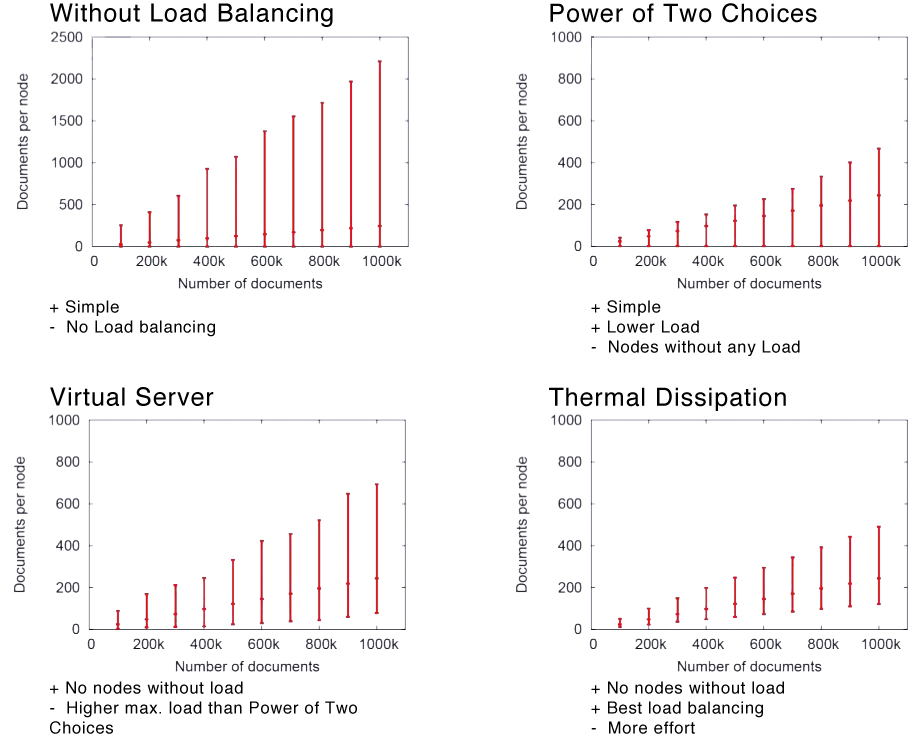
\includegraphics[width=1\textwidth]{img/lb.jpg}
  \caption{Load balancing approaches comparison}
  \label{fig:lbcomp}
\end{figure}


% paragraph load_balancing (end)

\paragraph{\textbf{Assurance and Trust}} % (fold)
\label{par:Assurance and Trust}

in a P2P network is an interesting challenge due to the lack of control over the machines that are willing to share with their resources, in order to achieve it, several strategies have been developed to maintain the integrity of the data using Cryptography, Reputation modeling schemes based on it's node previous record and also economic models, that resemble our own economy, but to share and trade computational resources.

Starting with the Cryptographic techniques, storage systems such as PAST give the option to the user to store encrypted content, disabling any other user, that does not have the encryption key, to have access to the content itself, this is a technique that comes from the Client-Server model, adapted to P2P environment, however, other cryptography technique benefits such as user authorization and identity, cannot be directly replicated into a P2P network without having a centralized authority to issue this validations, one of the alternatives is using distributed signature strategy, known as Threshold Cryptography \cite{Desmedt;1998}, where an access is granted if validated if several peers (a threshold), validates it's access, one implementation of Threshold Cryptography can be see in a P2P social network\cite{Afify} in order to guarantee privacy over the contents inside the network. 

Trust in a P2P system, as mentioned, is fundamental to it's well behaved functioning, not only in terms of data privacy, but also in giving the deserved resources to the executions that mostly need them, avoiding misbehaved peer intentions that can be a result of an Attack to jeopardize the network, one example is the known Sybil attack\cite{Douceura}. To achieve a fair trust sharing system, several metrics for a reputation mechanism have been developed \cite{Marti}, these can be seen in Table \ref{table:reputation}.

\begin{table}
  \centering
  \begin{tabular}{| c | c | c |}
    \hline                        
    \multicolumn{3}{|c|}{Reputation Systems} \\

    \hline                        
    Information Gathering & Scoring and Ranking & Response \\
    
    \hline                        
    Identity Scheme & Good vs. Bad Behavior & Incentives \\
    Info. Sources & Quantity vs. Quality & Punishment \\
    Info. Aggregation & Time-dependence &   \\ 
    Stranger Policy & Selection Threshold &   \\ 
      & Peer Selection &   \\ 

    \hline                           
  \end{tabular}
  \caption{Reputation system components and metric}
  \label{table:reputation}
\end{table}

Incentives for sharing resources\cite{Golle2001} can in the form of money rewards, greater speed access(used in Napster and some bittorrent networks) or it can be converted to a interchangeable rate to trade for more access to resources, giving the birth of economic models\cite{Filipe2011}\cite{Vishnumurthy}, that model the traded resources as a currency in which a peer has to trade in order to use the network.

% Economic Models
% * Gridlet Economics: Resource Management Models and Policies for Cycle-Sharing Systems
% * KARMA : A Secure Economic Framework for Peer-to-Peer Resource Sharing  (note: stores reputation remotly) Nead to Read


% paragraph Assurance and Trust (end)

% 
%---------{Resource sharing using the Web as platform}------------
% 
\subsection{Resource sharing using the Web platform} 

One of the main focuses with the proposed work, is to take advantage more recent developments of the Web platform, such as the high dynamic runtime that Javascript offers, the P2P browser capabilities enabled by WebRTC\cite{Google} in order to share resources for distributed computing and storage sharing. 

\subsubsection{3.3.1 Web Platform}

Since the introduction of AJAX\cite{Google/Mozzila/Opera} the web has evolved into a new state where it left being a place of static pages, known as Web 1.0, nowadays we can have rich web applications with degrees of interaction and levels of performance close to a native application. The programming languages that power the Web Platform, in special HTML, CSS and JavaScript\cite{Ecma2009}, have been suffering several changes, enabling `realtime' data transfers and fluid navigations through content. Javascript an interpreted language with an  high dynamic runtime has proven to be the right candidate for a modular Web Platform, enabling applications to evolve in a time continuum, by only changing the pieces of code that were updated.

\textbf{Emscripten}\cite{Zakai2011}, a LLVM(Low Level Virtual Machine) to JavaScript compiler, enabled native performance on Web apps by compiling any language that can be converted to LLVM bytecode, for example C/C++, into JavaScript. This tool enabled native game speed on the browser, where two of the major examples are the project Codename: ``BananaBread''\cite{Mozilla2012} and ``Epic Citadel''\cite{Mozilla2013}, in which Mozilla used Ecmascripten to port the entire Unreal Engine 3 to JavaScript. In Figure~\ref{fig:dan}, we can see a comparison of the performance of several algorithms, running on Dalvik, Android Java runtime, asm.js, the subset of Javascript that the code in C/C++ is transformed into when compiled with Emscripten and Native, the same C/C++ but running on a native environment. The results are very interesting, specially in the first test, where asm.js outperforms Native, the explanation towards this is due to the fact that BinaryTrees use a significant amount of `malloc', which is an expensive system call, where in asm.js, the code uses typedarrays, using `machine memory', which is allocated in the beginning of the execution once and used during the entire run.

\begin{figure}[h!]
  \centering
  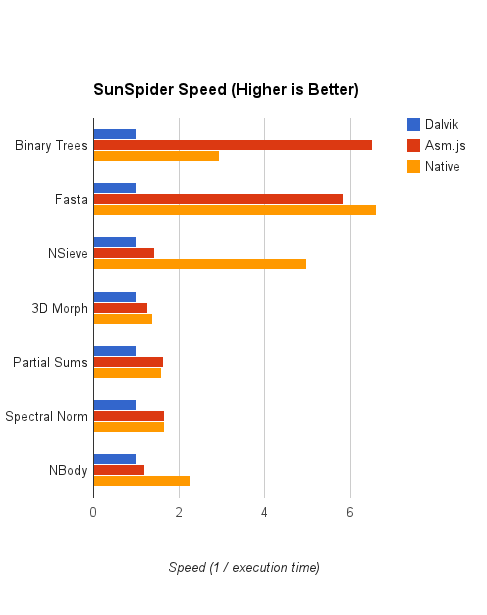
\includegraphics[width=0.82\textwidth]{img/Dalvik-vs-ASM-vs-Native-edited}
  \caption{Dalvik vs. ASM.js vs. Native performance}
  \label{fig:dan}
\end{figure}

\textbf{WebRTC}\cite{IanHickson2013}, a technology being developed by Google, Mozilla and Opera, with the goal of enabling Real-Time Communications in the browser via a JavaScript API. WebRTC brings to the browser the possibility of peer-to-peer interoperability. Peers perform their handshake through a `Signaling Server', the signaling server will exchange the `ICE(Interactive Connectivity Establishment) candidates' of each peer, this serve as an invite so a data-channel can be opened, a visualization of this process can be seen in Figure~\ref{fig:webrtc}. Since most of the browsers sit behind NAT, there is another server, named `Turn'(Relayw), which tell to each browser they public IP in the network. WebRTC, although being built with the goal of real-time voice and video communications, it has been shown as a viable technology do distribute content as seen in PeerCDN and SwarmCDN\cite{Vogt}.

\begin{figure}[h!]
  \centering
  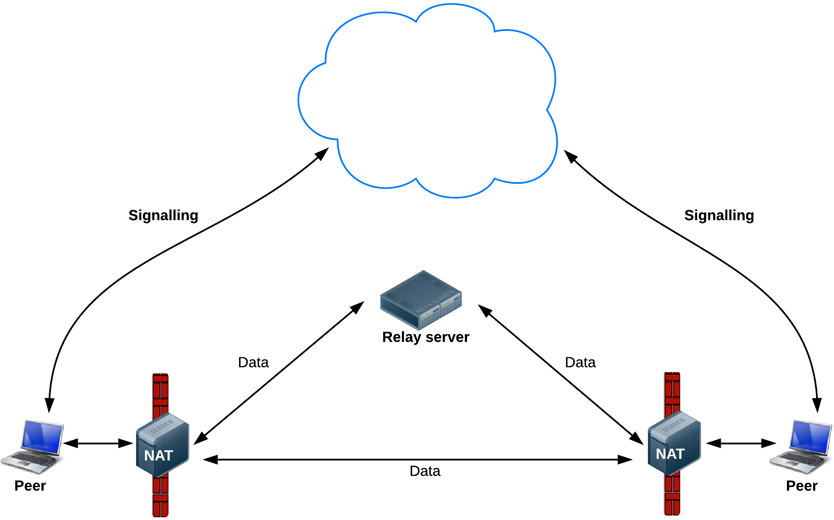
\includegraphics[width=0.95\textwidth]{img/webrtc.png}
  \caption{Example of a WebRTC session initiation}
  \label{fig:webrtc}
\end{figure}

% There is also Jingle
% https://github.com/legastero/jingle.js
% Jingle is an extension of XMPP that enables P2P and communication over RTC

\textbf{level.js} is an implementation of the leveldown API on top of IndexedDB, which in turn is implemented on top of the LevelDB, an open source on-disk key-value store inspired by Google BigTable 


% IndexedDB , Level JS
refs(notes to self):
http://www.w3.org/TR/IndexedDB/

https://code.google.com/p/leveldb/

https://npmjs.org/package/level-js

http://docs.basho.com/riak/latest/ops/advanced/backends/leveldb/


\textbf{HTTP 2.0} 
refs(notes to self):
http://http2.github.io/
% TODO HTTP 2.0




\subsubsection{3.3.2 Previous attempts on cycle sharing through web platform}
The first research of browser-based distributed cycle sharing was performed by Juan-J. Merelo, Juan Lupion and Fernando Tricas, which introduced a Distributed Computation on Ruby on Rails framework\cite{Merelo2007}. The system used a client-server architecture in which clients, using a browser would connect to a endpoint, where they would download the jobs to be executed and sent back the results. In order to increase the performance of this system, a new system\cite{Duda2013} of browser-based distributed cycle sharing was creating using Node.js as a backend for very intensive Input/Output operations\cite{Tilkov2010}, with the goal of increased efficiency, this new system uses normal webpages(blogs, news sites, social networks) to host the client code that will connect with the backend in order to retrieve and execute the jobs, while the user is using the webpage, this concept is known as parasitic computing\cite{Barabasi2001}, where the user gets to contribute with his resources without having to know exactly how, however since it's Javascript code running on the client, any user has access to what is being processed and evaluate if it presents any risk to the machine.


% ^^^^^^^^^^^^^^^^^^^^^^^^^^^^^^^^^^^^^^^^^^^^^^^^^^^^^^^^^^^^^^
% ~~~~~~~~~~~~~~~~~~~~~~~~~~~~~~~~~~~~~~~~~~~~~~~~~~~~~~~~~~~~~~
% ______________________________________________________________

% 
% Architecture
% 

\section{Architecture}

In this section it is described what is expected to be implemented. First, we present an overall of the architecture of Human's Cloud(Figure \ref{fig:overallarchitecture}), followed by a description of the individual components, responsible for separate tasks such as: developer front end (API), storage system, job scheduling techniques, the architecture of the system at the node level and finally, the proposed reputation system to assign different responsibilities for each Node.

\begin{figure}[h!]
  \centering
  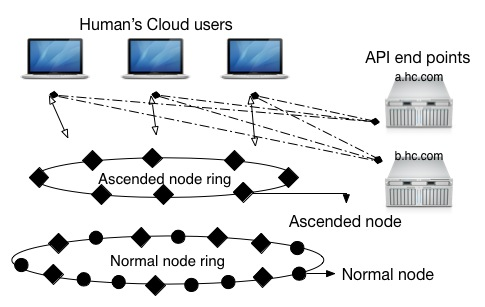
\includegraphics[width=0.7\textwidth]{img/overall.jpg}
  \caption{Human's cloud overall architecture}
  \label{fig:overallarchitecture}
\end{figure}

Human's Cloud proposed architecture has the goal of enabling the user to develop on top of computing and storage resources provided by volunteers, without having to change their current application conventions. 

Nodes (volunteer computers), are divided into two CHORD DHTs with the purpose of separating the nodes with storage responsibility from the ones with only computing responsibility. The reason behind this decision is due to the high churn rate in a P2P network, keeping the files in Nodes have proven to be more trustworthy for staying longer in the network makes the more robust by keeping the file replica level stable, this also reduces the message overhead that would require to keep the replica level in a more inconsistent environment. Never the less, the more volatile nodes are perfect for short computing operations, till they proven to be trustworthy to `ascend' in the network.

\subsection{Client API}

The client API offers the traditional and expected functions for a Cloud Computing services in a very Unix like way, which developers are familiar with, these are:

\begin{itemize}
   \item \textbf{\$ hcls}  - List files in a directory
   \item \textbf{\$ hccd}  - Traverse in storage directories   
   \item \textbf{\$ hcget} - Get an object stored
   \item \textbf{\$ hcput} - Store an object
   \item \textbf{\$ hcjob} - Initialize a job   
\end{itemize} 

In order to execute this commands, a `connect' action must be issued first in which the user will request to one of the API endpoints for one point of contact in the Ascended nodes ring, that will act as mediator for all the user communications. Human's Cloud provides several API end points as a fault tolerance mechanism, inspired by DNS, so the user has always a way to discover one node to contact.

To avoid node overload, the API endpoints have enabled a load balancing system that will assign different nodes as mediators to different users, based in the amount of activity the node was subjected too, the more activity, the less probability it will be selected next.

The creation of a job is described by a script, presenting the objects that will be manipulated and the several assets that will be used as steps in order to process the job, such as:

``hcjob create /path/to/files | step1 [| step2] | /path/to/output''

for example, if we are looking for video transcoding:

``hcjob create /path/to/file | ffmpeg | out.webm''
  
The assets, can be one of the present in Human' Cloud or one provided by the user, respecting the service policies of not using functionalities that may cause some misbehavior of the node executing the job. 


\subsection{Storage}

Human's Cloud storage happens in what it's named, the ``Ascended node ring'', this nodes have an higher reliability, making the storage system more stable, without the need of constantly burning computer cycles to maintain the files replica level.

Data stored in nodes can be:
\begin{itemize}
  \item File metadata (name of the file, size, location of the chunks, chunks hash).
  \item File chunks
  \item Directories metadata - This way, hcls can be more efficient 
  \item Job information (state, issuer, workflow)
  \item Reputation log
\end{itemize}

We classify storage nodes into two types, the `sKeeper', responsible for holding the metadata of the file and hashing each chunk to identify the `sHolder', nodes responsible to store the chunk into their system. This approach mitigates the possibility of having an high unbalanced storage distribution, diving each file in equal chunks across several nodes. As we can see in Figure~\ref{fig:chunking}, each chunk gets hashed more than one time with a different hash function, the purpose is to identify several Nodes that will be responsible to store a replica, also, in order to increase the fault tolerance of the system, we replicate the `sKeeper' responsibility in the 2 following nodes in the hashring, so if one of these fails, another is assigned.

\begin{figure}[h!]
  \centering
  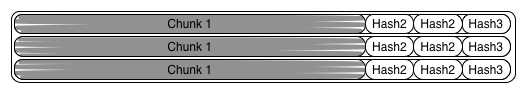
\includegraphics[width=0.7\textwidth]{img/chunking.jpg}
  \caption{A file partitioned in several chunks, each with its corresponding hashes that correspond to nodeIds}
  \label{fig:chunking}
\end{figure}

In Figure~\ref{fig:skeepersholder}, we can find the `sKeeper' and `sHolder' relationship. Only the sKeeper performs the chunk hashing and stores the information in the file lookup table, this happens one single time for each chunk, reducing several computer cycles for the consequent searches.

\begin{figure}[h!]
  \centering
  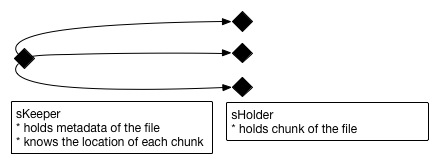
\includegraphics[width=0.7\textwidth]{img/skeepersholder.jpg}
  \caption{Representation of the Node responsible for the file(sKeeper) and it's individual chunk holders(sHolders)}
  \label{fig:skeepersholder}
\end{figure}

Each store file is chunked as soon as it enters the network, this mitigates the risk that would be present if we were transferring files with considerable sizes all at once, starving the network and the node's heap. The only point where the file gets glue together again is when it leaves the network and sent to the user.

Human's Cloud adapts the Load Balancing virtual server's method, by using the same strategy of global load, but by transferring files between sHolders and not an entire virtual server, updating the respective sKeeper accordingly. The reasons behind

Files are storage as objects in a indexedDB type storage, provided by the leveljs module. 

\subsection{Job Scheduling}

One of the challenges that Human's cloud propose to solve is the job coordination in a completely distributed environment, in a sustainable scalable way. Traditionally in the client-server model, we have the possibility to select one of the nodes to be the job coordinator, to implement this in a P2P network, we take advantage of the DHT, to select randomly one of the ascended nodes to be the `jKeeper', the node responsible for coordinating the job in an environment a P2P network.

The `jKeeper', is responsible for contacting the `sKeepers' of each individual file, and coordinate them to command each of `sHolder' to perform the desired computation on the file.

All the steps during the computation are journaled in the Job log, store with the coordinator, and replicated in the 2 following nodes for Fault Tolerance measure.

All the coordination happens in the ascended Node ring, however, in order to take advantage of the normal node ring resources, `sHolders' are allowed to offload the computation to process this job in the `normal hash ring', this is done by sending a probe, asking for `volunteers' for a job, when the threshold required is met, the orchestration starts, where the `sHolder' transfers the data and the assets necessary for processing it.


% TODO Fazer aqui um boneco

% note como processar ficheiros que dependem de todos os chunks, not :)

\subsection{Node Level}

At the node level, we divide the application into two fundamental services and 3 pluggable components, with the possibility for expansion, thanks to Javascript dynamic runtime, we can find this structure in Figure~\ref{fig:hcnode}.

Starting with the communication layer, where the DHT logic is implemented, where the functional calls to propagate messages through the hash ring are implemented. 

Next, we have the Service Routing layer, this service is responsible to guide the message to the right component, this enables the architecture to be more modular, plugging in more components as it's needed, for example, when a node ascends and needs the storage component to fulfill his responsibility.

Last, we have the components, individual modules that do one thing and one thing well. Currently, we present the Storage module, responsible for holding the data, the Job Schedule, responsible to orchestrate jobs issued by the users, the assets needed to execute the jobs and finally the job executor, the module that will execute the jobs in a separate process using webworkers.

% Doug McIlroy, then head of the Bell Labs CSRC and contributor to Unix pipes,[1] summarised Unix philosophy as follows:[2]
% This is the Unix philosophy: Write programs that do one thing and do it well. Write programs to work together. Write programs to handle text streams, because that is a universal interface.

\begin{figure}[h!]
  \centering
  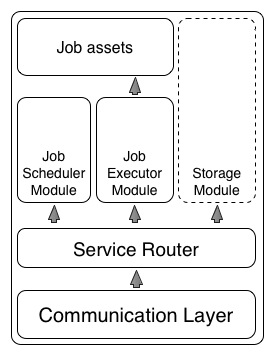
\includegraphics[width=0.35\textwidth]{img/node.jpg}
  \caption{Human's Cloud Node}
  \label{fig:hcnode}
\end{figure}

\subsection{Reputation Mechanism}

The reputation mechanism present will enable the network to identify the nodes that show more availability and have the necessary means to ascend and take a more important role. In order to evaluate each node, we define several metrics, these are: uptime, number of job completions, network throughput and  computational resources available, being the uptime, the most important, to assure stability.

The reputation of each node is stored with its node identifier on the `ascended hash ring', each time a job is completely successfully, his score gets updated and in case it reaches the required level to ascend, the jKeeper that was updating his score will enable and deploy the remaining features(storage and job schedule module) he needed to join the ascended group. 


% ^^^^^^^^^^^^^^^^^^^^^^^^^^^^^^^^^^^^^^^^^^^^^^^^^^^^^^^^^^^^^^
% ~~~~~~~~~~~~~~~~~~~~~~~~~~~~~~~~~~~~~~~~~~~~~~~~~~~~~~~~~~~~~~
% ______________________________________________________________

% 
% Evaluation
% 

\section{Evaluation}

The proposed system will be evaluated having into consideration the several dimensions that will define its ability to provide a reliable storage, following the CAP theorem(Consistency , Availability and Partition Tolerant), adding also as criteria, its latency and speed while performing distributed jobs over the stored data.

\subsection{Evaluation of the data consistency, availability and partition tolerant}

Data consistency will be implicitly granted by having an put/delete system only, since an update to a file means rewriting the file again, a new ID will be created and by doing so, a new sKeeper is elected, avoiding a distributed lock or conflict over the same id of file. Never the less, availability and partition tolerance must be evaluated, having in consideration the hostility of environment, we want to prove that Nodes considered trustworthy(ascended), are in fact enough to guaranteed the necessary availability for any given file at any given time and that the replica number can keep stable without generating too much message overhead. To prove this, resilience will be put into test by varying the churn rate with several usage scenarios, for example, a surge.

This tests will be executed in two different stages, the first one, ``in lab'', will be a controlled P2P environment, where different browsers and computers will be used for tests, in order to evaluate and calculate the factors that are used to calculate values such as: reputation, threshold to ascend one Node and block size. 

After realizing how the system can perform best, a ``field'' trial will be executed, this will be executed by approaching volunteers that might want to contribute to the experiment, loading the code into their browser so real world tests can be performed.

\subsection{Evaluation of latency when storing, fetching and jobs execution}

To prove that the system is app development ready, we need to optimize and verify how much performant it behaves, this will enable for it's users to know before hand how it stacks to current cloud systems using a more traditional approach. To evaluate and identify how the system behaves, several tests will be executed during the ``in lab'' and ``field'' experiments, varying the load, the complexity of the job, the churn rate and the number of nodes.


% ^^^^^^^^^^^^^^^^^^^^^^^^^^^^^^^^^^^^^^^^^^^^^^^^^^^^^^^^^^^^^^
% ~~~~~~~~~~~~~~~~~~~~~~~~~~~~~~~~~~~~~~~~~~~~~~~~~~~~~~~~~~~~~~
% ______________________________________________________________

% 
% Conclusions
% 

\section{Conclusions}

We end this article, making an overview and summing up all the primary aspects of the proposed work and how it relates to what has been researched so far, presenting also some concluding remarks.
People sharing resources is one of the oldest sociological behaviors in human history, however although some known attempts as SETI@HOME have enabled that for our computer machinery, the level of friction that has to be made in order for a user to join, has been significantly high to cause a great user adoption, in the other hand, Open Cloud stacks have been evolving, providing nowadays the most reliable and distributed systems performance, having a bigger adoption even if the resources are geographically more distant or expensive.
The proposed work is an exercise to work towards a federated community cloud that will enable its users to share effectively their resources, giving the developers a reliable and efficient way to store and process data for their applications, with an API thats familiar to the centralized Cloud model.

% ^^^^^^^^^^^^^^^^^^^^^^^^^^^^^^^^^^^^^^^^^^^^^^^^^^^^^^^^^^^^^^
% ~~~~~~~~~~~~~~~~~~~~~~~~~~~~~~~~~~~~~~~~~~~~~~~~~~~~~~~~~~~~~~
% ______________________________________________________________


% 
% Acronym List
% 

% \acrodef{P2P}{peer-to-peer}
% % \acro{abc}[short version]{full version}
% % \acro{efd}[shortAAA version]{full AAAversion}


% ^^^^^^^^^^^^^^^^^^^^^^^^^^^^^^^^^^^^^^^^^^^^^^^^^^^^^^^^^^^^^^
% ~~~~~~~~~~~~~~~~~~~~~~~~~~~~~~~~~~~~~~~~~~~~~~~~~~~~~~~~~~~~~~
% ______________________________________________________________

% 
% Bibliography
% 

\bibliographystyle{plain} 
\bibliography{/Users/DavidDias/Documents/bibtex/THESISREAD.bib}
\end{document}